%%%%%%%%%%%%%%%%%%%%%%% file template.tex %%%%%%%%%%%%%%%%%%%%%%%%%
%
% This is a general template file for the LaTeX package SVJour3
% for Springer journals.          Springer Heidelberg 2010/09/16
%
% Copy it to a new file with a new name and use it as the basis
% for your article. Delete % signs as needed.
%
% This template includes a few options for different layouts and
% content for various journals. Please consult a previous issue of
% your journal as needed.
%
%%%%%%%%%%%%%%%%%%%%%%%%%%%%%%%%%%%%%%%%%%%%%%%%%%%%%%%%%%%%%%%%%%%
%
% First comes an example EPS file -- just ignore it and
% proceed on the \documentclass line
% your LaTeX will extract the file if required
\begin{filecontents*}{example.eps}
%!PS-Adobe-3.0 EPSF-3.0
%%BoundingBox: 19 19 221 221
%%CreationDate: Mon Sep 29 1997
%%Creator: programmed by hand (JK)
%%EndComments
gsave
newpath
  20 20 moveto
  20 220 lineto
  220 220 lineto
  220 20 lineto
closepath
2 setlinewidth
gsave
  .4 setgray fill
grestore
stroke
grestore
\end{filecontents*}
%
\RequirePackage{fix-cm}
%
%\documentclass{svjour3}                     % onecolumn (standard format)
%\documentclass[smallcondensed]{svjour3}     % onecolumn (ditto)
%\documentclass[smallextended]{svjour3}       % onecolumn (second format)
\documentclass[twocolumn]{svjour3}          % twocolumn
%
\smartqed  % flush right qed marks, e.g. at end of proof
%
\usepackage{graphicx}
\newcommand{\etal}{\textit{et al}. }

\begin{document}

\title{Wildland Fire Modeling Using Convolutional Neural Networks
}

\author{Jonathan L. Hodges         \and
        Brian Y. Lattimer
}

\institute{J. L. Hodges \at
              Jensen Hughes\\
              2020 Kraft Drive, Suite 3020\\
              Blacksburg, VA 24060 USA \\
              Tel.: +1 540-808-2800 x10611\\
              \email{jhodges@jensenhughes.com}
}

\date{Received: date / Accepted: date}
% The correct dates will be entered by the editor


\maketitle

\begin{abstract}
Insert your abstract here. Include keywords, PACS and mathematical
subject classification numbers as needed.







\keywords{Wildland Fire \and  Machine Learning \and Neural Network \and Fire Spread}
% \PACS{PACS code1 \and PACS code2 \and more}
% \subclass{MSC code1 \and MSC code2 \and more}
\end{abstract}




\section{Introduction}
\label{intro}

Wildland fire propagation is a complex process which involves the
interactions of many underlying physical phenomena. Since fully
resolving these processes remains a research effort; quasi-empirical
fire spread models are often used to predict spread across large domains
\cite{sullivan2007a}. Quasi-empirical models are based on fitting experimental
measurements to an expected functional form \cite{sullivan2007b}, such
as the model of Rothermel \cite{rothermel1972mathematical,scott2005standard} which uses
empirical correlations for heat source and sink terms in
conservation of energy \cite{weber1991modelling}. Difficulties arise when
modeling complex scenarios which do not fit the functional form for
which the quasi-empirical model was developed. One of the key advantages
of applying machine learning is the capacity of the model to learn an underlying
functional form.

Several researchers have applied machine learning algorithms to predict the total burned area of a fire based on
meteorological data.
Safi \etal used a deep feed-forward neural network with the Montesinho Natural Park data set (MNP) \cite{safi2013prediction}.
Castelli \etal compared total burned area estimates using multiple machine learning algorithms (genetic programming, random forests, feed-forward neural network, etc.) with MNP \cite{castelli2015predicting}.
Storer \etal improved the estimates using a feed-forward neural network by training the weights using Particle Swarm Optimization with MNP \cite{storer2016pso}.
Naganathan \etal compared support vector machines, k-nearest neighbors, and decision trees burned area predictions of US fires trained with MNP \cite{naganathan2016wildfire}.
Cao \etal compared burned area predictions using logistic regression, feed-forward neural network, and random forest algorithms with Yunnan Province fire data \cite{cao2017wildfire}.
These models have been limited to total burned area predictions, which will not capture the spatial-temporal distribution of the fire front.

%Several researchers have investigated using machine learning in forest research
%management \cite{peng1999recent,imada2014literature}.
%Sakr \etal used support vector machines based on daily meteorological measurements and seasonal precipitation estimates to assess fire risk \cite{sakr2010artificial}.

McCormick developed a quasi-empirical fire spread model which used predictions
from a feed-forward neural network to propagate the fire front \cite{mccormick2001toward,mccormick2002developing}.
The model considers a 3x3 neighborhood of pixels to classify the center pixel as burned
or unburned. The order pixels are considered is based on the fire growth
modeling by Finney which considers an ellipsoidal growth profile in the direction of wind
\cite{finney1999mechanistic}. The results shown good spatial agreement between predicted and
known fires. One limitation of this model is the inability to predict the time-resolved
fire front. The author used pixels from all 11 fires to predict each of the fires which
begs the question how well the model would predict a fire which none of the pixels were
used to train the network.

%O'Connor \etal used a boosted regression tree to predict final boundary will be of an active fire.

The objective of this study is to develop a fire spread model using a convolutional
neural network which accurately predicts the spatial-temporal distribution of the
fire front in a wildland fire. Sensitivity of the network to each input parameter is 
examined. The trained parameters of the network are used to
infer relationships about input parameters. 






\section{Methods}
\label{s:Methods}

Wildland fires


\subsection{Wildland Fire Prediction}
\label{ss:Wfp}

Description goes here.


\subsection{Convolutional Neural Networks}
\label{ss:Cnn}

Description goes here.


\subsection{Network Architecture}
\label{ss:Na}

Description goes here.



\subsection{Data Pre-Processing}
\label{ss:Dpp}

Description goes here.



\section{Results}
\label{s:Results}

Cool pictures go here.



\section{Discussion}
\label{s:Discussion}

Talk about what the resutls show us and why the readers should care.




\section{Conclusion}
\label{s:Conclusion}

Summarize impact of the work.




% For one-column wide figures use
\begin{figure}
% Use the relevant command to insert your figure file.
% For example, with the graphicx package use
  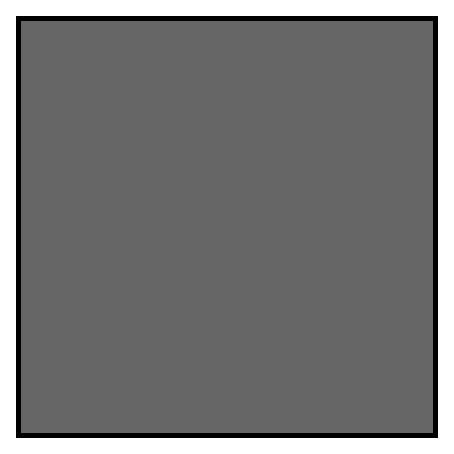
\includegraphics{example.eps}
% figure caption is below the figure
\caption{Please write your figure caption here}
\label{fig:1}       % Give a unique label
\end{figure}
%
% For two-column wide figures use
\begin{figure*}
% Use the relevant command to insert your figure file.
% For example, with the graphicx package use
  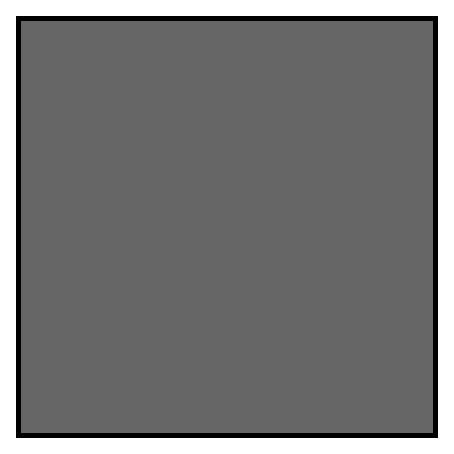
\includegraphics[width=0.75\textwidth]{example.eps}
% figure caption is below the figure
\caption{Please write your figure caption here}
\label{fig:2}       % Give a unique label
\end{figure*}
%
% For tables use
\begin{table}
% table caption is above the table
\caption{Please write your table caption here}
\label{tab:1}       % Give a unique label
% For LaTeX tables use
\begin{tabular}{lll}
\hline\noalign{\smallskip}
first & second & third  \\
\noalign{\smallskip}\hline\noalign{\smallskip}
number & number & number \\
number & number & number \\
\noalign{\smallskip}\hline
\end{tabular}
\end{table}


%\begin{acknowledgements}
%If you'd like to thank anyone, place your comments here
%and remove the percent signs.
%\end{acknowledgements}

% BibTeX users please use one of
%\bibliographystyle{spbasic}      % basic style, author-year citations
%\bibliographystyle{spmpsci}      % mathematics and physical sciences
\bibliographystyle{spphys}       % APS-like style for physics
\bibliography{wildfireReferences}   % name your BibTeX data base

% Non-BibTeX users please use
%\begin{thebibliography}{}
%
% and use \bibitem to create references. Consult the Instructions
% for authors for reference list style.
%
%\bibitem{weber1991}
%Rodney O. Weber, Modelling fire spread through fuel beds, Progress in Energy and Combustion Science, 17, 67-82 (1991)
%\bibitem{rothermel1972}
%Richard C. Rothermel, A mathematical model for predicting fire spread in wildland fuels, U.S. Department of Agriculture, Forest Service, Ogden, UT (1972)
%\bibitem{scott2005}
%Joe H. Scott; Robert E. Burgan, Standard fire behavior fuel models: a comprehensive set for use with Rothermel's surface fire spread model, U.S. Department of Agriculture, Forest Service, Rocky Mountain Research Station, Fort Collins, CO (2005)

% Format for books
%\bibitem{RefB}
%Author, Book title, page numbers. Publisher, place (year)
%\end{thebibliography}

\end{document}

